\documentclass{beamer}
\usepackage{beamerthemeshadow}
\usepackage{graphicx}
\usepackage{color}
\usepackage{xcolor}
\usepackage[utf8]{inputenc}
\usepackage[serbian]{babel}
\usepackage{cmsrb}
\usepackage{hyperref}
\usepackage{caption}
\usepackage[flushleft]{threeparttable}
\usepackage{subfigure}
\setbeamercolor{structure}{fg=blue}
\captionsetup[figure]{labelformat=empty}
\captionsetup[table]{labelformat=empty}


\def\d{{\fontencoding{T1}\selectfont\dj}}
\def\D{{\fontencoding{T1}\selectfont\DJ}}


\title{Tehničko i naučno pisanje}
\subtitle{-- IT konferencije u Srbiji 2022. godine --}
\author{Nevena Jokić \and Andrej Mihajlov\\ \and Jovan Gagić \and Dušan Lukić}
\institute{Matematički fakultet\\Univerzitet u Beogradu}
\date{
	\footnotesize{Beograd, 2023.}	
}

\begin{document}
\begin{frame}
	\thispagestyle{empty}
	\titlepage
\end{frame}

\addtocounter{framenumber}{-1}

\begin{frame}[fragile]\frametitle{Literatura}
	\begin{itemize}
		\item Zasnovano na seminarskom radu "IT Konferencije u Srbiji 2022. godine - Nevena Jokić, Andrej Mihajlov, Jovan Gagić, Dušan Lukić", koji se može naći na sledećem linku:
		(\url{https://github.com/nejviblue/42_TNP2022/blob/main/42_TNP2022.pdf})
	\end{itemize}
\end{frame}

\begin{frame}
	\frametitle{Sadržaj}
	\tableofcontents[] 
\end{frame}
\section{Uvod}

\subsection{Istorijat}

\begin{frame}[fragile]\frametitle{Uvod}
	\begin{itemize}	
		\item Konferencije su planirani događaji na kojima se profesionalci ili stručnjaci okupljaju kako bi podelili znanje, razmenili ideje i povezali se sa drugima u istoj oblasti.
		\item IT konferencije su konferencije koje za cilj imaju da okupe stručnjake i istraživače iz polja informacionih tehnologija kao i ljude koji žele da nauče više o njima. Učesnici se okupljaju da diskusuju o novim idejama, trendovima i razvoju IT sektora.
       \item  Srbija, kao zemlja koja sve više prepoznaje potencijal informacionih tehnologija, postala je i 2022. godine domaćin raznovrsnim i velikim IT konferencijama koje su okupile stručnjake i znatiželjne iz celog sveta.
	\end{itemize}
\end{frame}

\subsection{TELFOR 2022}

\begin{frame}[fragile]\frametitle{TELFOR 2022}
	\begin{itemize}	
		\item Telekomunikacioni forum TELFOR je internacionalni godišnji skup stručnjaka koji rade u oblastima telekomunikacija i informacionih tehnologija.
		\item Tipično, na Telfor dolazi oko 2000 posetilaca i za TELFOR se prihvata od 300-500 detaljno recenziranih radova sa ukupno 700-900 autora/koautora.
	\end{itemize}
\end{frame}


\subsection{Sinergija 2022}
\begin{frame}[fragile]\frametitle{Sinergija 2022}
\begin{itemize}
    \item Sinergija je jedna od najvećih i najuticajnijih konferencija u Jugoistočnoj Evropi posvećena digitalnoj transformaciji.
    \item Organizuje je Microsoft Srbija i održava se već 22 godine.
    \item U tabeli \ref{tab:tabela1} su prikazane statistike za Sinergiju 22, odnosno koliko je bilo izlagača, posteilaca i veličina izložbenog prostora.
\end{itemize}
\begin{table}[h!]
\begin{center}
\begin{tabular}{|ccc|} \hline
\multicolumn{3}{|c|}{Statistike za Sinergiju 22}                                                                  \\ \hline
\multicolumn{1}{|c|}{Broj izlagača} & \multicolumn{1}{c|}{Broj posetilaca}          & Izložbeni prostor          \\ \hline
\multicolumn{1}{|c|}{90+}      & \multicolumn{1}{c|}{2000+} &  Crowne plaza Beograd \\ \hline
\end{tabular}
\caption{Statistika za Sinergiju 22}
\label{tab:tabela1}
\end{center}
\end{table}

\end{frame}



\subsection{TMRW Belgrade konferencija}
\begin{frame}[fragile]\frametitle{TMRW Belgrade konferencija}

\begin{itemize}
    \item TMRW konferencija je jedna od najvećih tehnoloških događaja u usponu u Evropi koja okuplja preko 40000 učesnika, kako uživo tako i online, kao i preko 100 govornika i prezentatora.
    \item Glavna tema ove konferencije je istraživanje najnovijih trendova u oblastima veštačke inteligencije, blokčejna, kriptovaluta, NFT -ja, metavers-a i gejminga kao i upoznavanje učesnika sa istim.
    \item 2022. je bilo više od 50 govornika i uvodnih izlaganja sa brojnim interaktivnim disusijama i radionicama.
\end{itemize}

\end{frame}
\subsection{19. COMING IT}
\begin{frame}[fragile]\frametitle{19. COMING IT}

\begin{itemize}
    \item Kompanija COMING, jedan od lidera u ICT oblasti u Srbiji i regionu, je kompanija koja postavlja za cilj kreiranje, razvijanje i pružanje IT sistema i usluga.
    \item 25. oktobra 2022. godine organizovali su svoju 19. IT konferenciju.
    \item Na slici \ref{fig:agar} se vidi robot AGAR koji se prikazao tokom uvodne sesije konferencije.
\end{itemize}

\begin{figure}[h!]
        \centering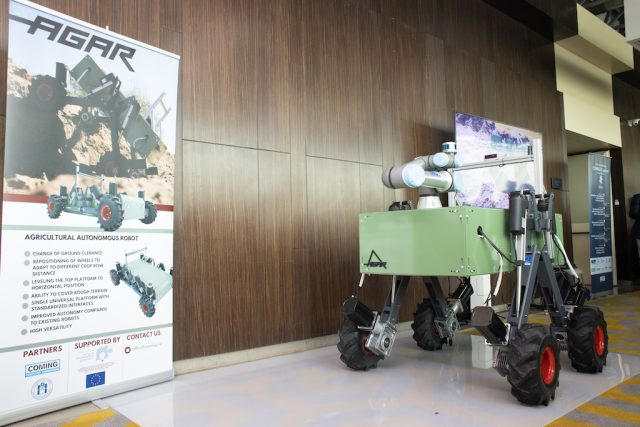
\includegraphics[height=2.5cm]{slike/agar.jpg} 
        \caption{Demonstracija AGAR-a – Universal agriculture autonomous robot, poljoprivrednog robota.}
        \label{fig:agar}
\end{figure}

\end{frame}

\subsection{Data Science Conference 2022}
\begin{frame}[fragile]\frametitle{Data Science Conference 2022}

\begin{itemize}
    \item DataScienceConference je internacionalna AI i Data konferencija u Beogradu koja pruža najsavremenije uvide u AI i Data Science.
    \item 2022. godine je bilo preko 200 govora i 50 tech tutorijala.
    \item Govornici na ovoj konferenciji dolaze iz nekih od najuticajnijih IT kompanija na svetu poput Google, IBM, VMWare i EyeSee.

\end{itemize}

\end{frame}

\subsection{Open IT}
\begin{frame}[fragile]\frametitle{Open IT}

\begin{itemize}
    \item Open IT je najveća IT konferencija za mlade.
    \item U dva dana konferencije na jednom mestu okupljaju 350+ mladih, 10+ govornika i 40+ predavača iz 20+ kompanija.
    \item Na slici \ref{fig:openit} se vide učesnici u FON-ovom amfiteatru
\end{itemize}

\begin{figure}[h!]
        \centering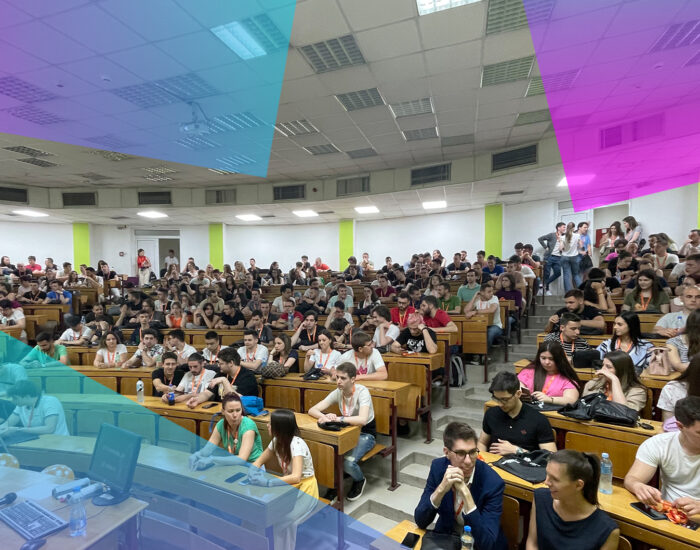
\includegraphics[height=2.5cm]{slike/openit.jpg} 
        \caption{Učesnici konferencije u FON-ovom amfiteatru}
        \label{fig:openit}
\end{figure}


\end{frame}

\section{Zaključak}

\begin{frame}[fragile]\frametitle{Zaključak}
\begin{itemize}
    \item Konferencije su postale važan deo društva i profesionalnog razvoja kompanija, posla i ljudi.
    \item Omogućavaju učesnicima da se povežu sa stručnjacima i kolegama iz celog sveta.
    \item Razmenjuju se mišljenja, ideje, iskustva, naučni radovi i još mnogo drugih stvari koje pomažu pojedincima u izgradnji odnosa i novih tehnologija.
    \item Srbija, iako ne spada među velike države, je svejedno često domaćin velikim IT dešavanjima i konferencijama. Stotine ljudi, a pogotovo mladi, iz regiona i sveta dolaze u Beograd da učestvuju u raznim IT radionicama koje ove konferencije organizuju.
	\end{itemize}
\end{frame}

\end{document}